\documentclass[border=5pt]{standalone}
\usepackage{graphicx}
\usepackage{xcolor}
\usepackage{tikz}
\usetikzlibrary{arrows.meta,calc,backgrounds}

\definecolor{pvoBlue}{HTML}{2F6FED}
\definecolor{pvoGreen}{HTML}{2AA876}
\definecolor{pvoRed}{HTML}{E05252}
\definecolor{pvoPurple}{HTML}{7C3AED}

\tikzset{
    module/.style={inner sep=0pt, outer sep=2pt},
    flow/.style={-{Latex[length=1.8mm]}, line width=0.9pt, draw=black!62},
    riskflow/.style={-{Latex[length=1.8mm]}, line width=1.0pt, draw=pvoRed!78!black},
    trainflow/.style={-{Latex[length=1.8mm]}, line width=0.9pt, draw=pvoBlue!78!black},
    deployflow/.style={-{Latex[length=1.8mm]}, line width=0.9pt, dashed, draw=pvoGreen!75!black},
    updateflow/.style={-{Latex[length=1.7mm]}, line width=0.8pt, dashed, draw=pvoBlue!70!black},
    labeltext/.style={font=\sffamily\tiny, fill=white, inner sep=1.2pt, text=black!68}
}

\begin{document}
\begin{tikzpicture}[font=\sffamily\scriptsize]
    % Observation and branch encoders.
    \node[module] (lidar) at (0.95,6.25)
        {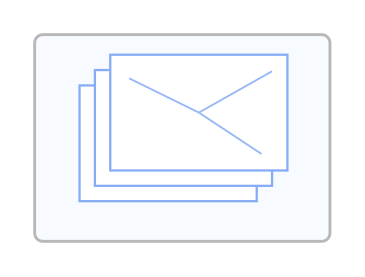
\includegraphics[width=1.90cm]{01_lidar_sequence.png}};
    \node[module] (state) at (0.95,4.95)
        {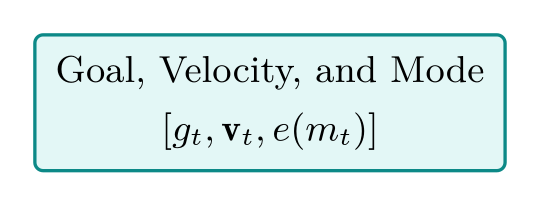
\includegraphics[width=1.82cm]{02_robot_state.png}};
    \node[module] (lidarenc) at (3.05,6.25)
        {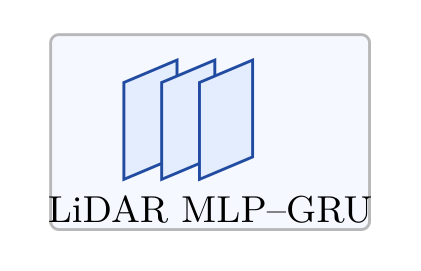
\includegraphics[width=1.85cm]{03_lidar_encoder.png}};
    \node[module] (stateenc) at (3.05,4.95)
        {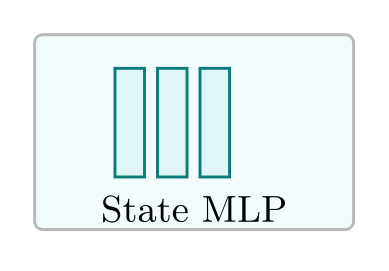
\includegraphics[width=1.70cm]{04_state_encoder.png}};
    \node[module] (fusion) at (4.95,5.60)
        {
\includegraphics[width=1.12cm]{05_fused_embedding.png}};

    % Risk-aware deployment chain.
    \node[module] (actor) at (4.95,3.55)
        {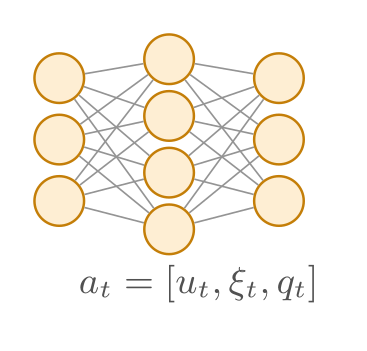
\includegraphics[width=1.72cm]{06_td3_actor.png}};
    \node[module] (pvo) at (6.95,3.55)
        {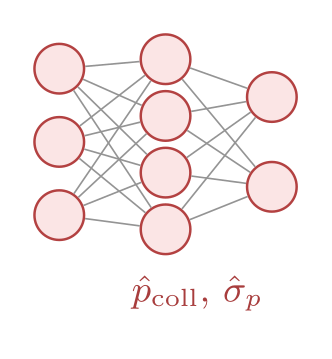
\includegraphics[width=1.58cm]{08_neural_pvo.png}};
    \node[module] (filter) at (8.70,3.55)
        {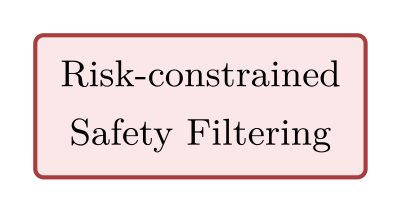
\includegraphics[width=1.42cm]{09_safety_filter.png}};
    \node[module] (mapper) at (10.58,3.55)
        {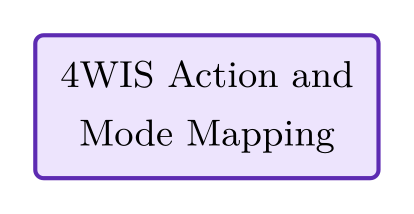
\includegraphics[width=1.64cm]{10_4wis_mapper.png}};
    \node[module] (velocity) at (12.55,3.55)
        {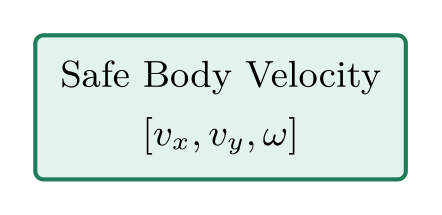
\includegraphics[width=1.72cm]{11_safe_velocity.png}};
    \node[module] (gazebo) at (14.85,3.55)
        {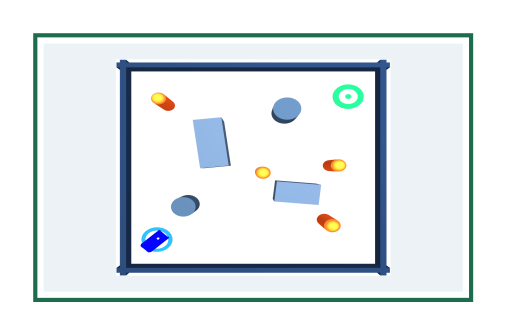
\includegraphics[width=2.22cm]{15_gazebo_validation.png}};

    % IRSim training feedback.
    \node[module] (critic) at (4.95,0.92)
        {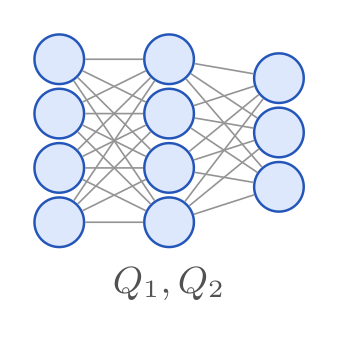
\includegraphics[width=1.48cm]{07_td3_critic.png}};
    \node[module] (reward) at (7.05,0.92)
        {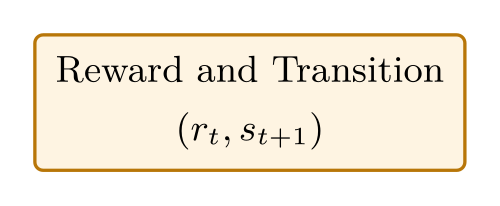
\includegraphics[width=1.58cm]{14_reward_transition.png}};
    \node[module] (irsim) at (9.35,0.92)
        {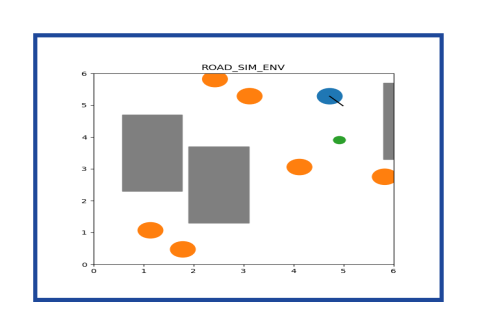
\includegraphics[width=1.92cm]{13_irsim_training.png}};
    \node[module] (proxy) at (8.70,2.20)
        {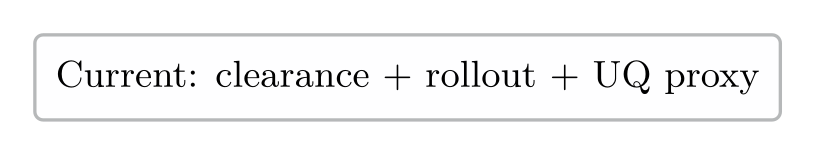
\includegraphics[width=1.94cm]{12_geometry_proxy.png}};

    \begin{scope}[on background layer]
        \draw[flow] (lidar.east) -- (lidarenc.west);
        \draw[flow] (state.east) -- (stateenc.west);
        \draw[flow] (lidarenc.east) -- (fusion.north west);
        \draw[flow] (stateenc.east) -- (fusion.south west);
        \draw[flow] (fusion.south) -- (actor.north);
        \draw[riskflow] (actor.east) -- (pvo.west);
        \draw[riskflow] (pvo.east) -- (filter.west);
        \draw[flow] (filter.east) -- (mapper.west);
        \draw[flow] (mapper.east) -- (velocity.west);
        \draw[deployflow] (velocity.east) -- (gazebo.west);

        \draw[trainflow] (irsim.west) -- (reward.east);
        \draw[trainflow] (reward.west) -- (critic.east);
        \draw[updateflow] (critic.north) -- (actor.south);
        \draw[densely dashed, line width=0.75pt, draw=black!45]
            (proxy.north) -- (filter.south);
    \end{scope}

    \node[labeltext, text=pvoBlue!72!black] at (5.22,2.25) {policy update};
    \node[font=\sffamily\tiny, text=pvoRed!72!black, align=center]
        at (6.95,2.58) {history- and action-conditioned\\future collision inference};

    \node[font=\sffamily\bfseries\small, text=black!70] at (2.55,7.18)
        {Observation and Feature Extraction};
    \node[font=\sffamily\bfseries\small, text=pvoRed!75!black] at (10.20,4.52)
        {Risk-aware Deployment Pipeline};
    \node[font=\sffamily\bfseries\small, text=pvoBlue!75!black] at (7.20,-0.28)
        {IRSim Actor--Critic Training Loop};
\end{tikzpicture}
\end{document}
